\documentclass[11pt,a4paper]{article}
\usepackage{fontspec}
\usepackage{polyglossia}
\setdefaultlanguage{russian}
\setotherlanguage{english}
\setmainfont{Times New Roman}
\setsansfont{Arial}
\setmonofont{PT Mono}
\newfontfamily\cyrillicfonttt{PT Mono}
\usepackage{amsmath,amssymb,mathtools}
\usepackage[margin=22mm,bottom=21mm]{geometry}
\usepackage{graphicx,booktabs,array,caption,enumitem}
\usepackage{xcolor}
\usepackage{xurl}
\usepackage[colorlinks=true,linkcolor=black,urlcolor=blue!45!black]{hyperref}
\usepackage{fancyhdr}
\usepackage{setspace}
\setstretch{1.12}
\setlength{\parskip}{4pt}
\emergencystretch=2em
\setlength{\parindent}{1.1em}
\setlength{\headheight}{15pt}
\pagestyle{fancy}
\fancyhf{}
\fancyhead[L]{\small Суперкомпьютерное моделирование и технологии}
\fancyhead[R]{\small Задача 1, вариант 12}
\fancyfoot[C]{\thepage}
\renewcommand{\headrulewidth}{0.3pt}
\captionsetup{font=small,labelfont=bf,hypcap=false}
\setlist{nosep,leftmargin=1.5em}
\newcommand{\norm}[1]{\left\lVert #1\right\rVert}
\newcommand{\E}{\mathrm{E}}
\newcommand{\grid}[2]{#1\!\times\!#2}
\graphicspath{{figures/}}
\hypersetup{pdftitle={Задача 1, вариант 12: метод фиктивных областей и параллельный CG},pdfauthor={Доронин Александр Константинович}}
\begin{document}
\begin{titlepage}
\centering
{\large Московский государственный университет имени М. В. Ломоносова\par}
\vspace{0.3cm}
{\large Факультет вычислительной математики и кибернетики\par}
\vspace{2.2cm}
{\Large\bfseries Отчёт по практикуму\par}
\vspace{0.5cm}
{\Large «Суперкомпьютерное моделирование и технологии»\par}
\vspace{0.9cm}
{\LARGE\bfseries Решение задачи Дирихле\par в криволинейной области\par}
\vspace{0.7cm}
{\large Задача 1, вариант 12\par}
{\large Метод фиктивных областей. Последовательная,\par OpenMP, MPI и MPI+OpenMP реализации\par}
\vspace{1.7cm}
\begin{flushright}
Выполнил: Доронин Александр Константинович\\
Группа 609
\end{flushright}
\vfill
\begin{minipage}{0.94\textwidth}
\small
Исходный код, тесты, протоколы и исходник отчёта:\\
\url{https://github.com/Shirlineyn/skipod-task1-2026}

Основная реализация расположена в ветке \texttt{main}; дополнительная
MPI+CUDA-реализация сохранена в ветке \texttt{cuda}. Использование ИИ и
границы проведённых проверок раскрыты в конце отчёта.
\end{minipage}
\vspace{1cm}

Москва, 3 ноября 2026 года
\end{titlepage}

\section{Постановка задачи и разностная схема}
Требуется решить задачу Дирихле
\begin{equation}
-\Delta u=1\quad\text{в }D,\qquad u=\sin(x+y)\quad\text{на }\partial D,
\end{equation}
где для варианта 12
\[
D=\{(x,y):x^2-4y^2>1,\ 1<x<3\}.
\]
Область ограничена правой ветвью гиперболы $x=\sqrt{1+4y^2}$ и отрезком
$x=3$, $|y|\leq\sqrt2$. Площадь равна
\[
|D|=\int_{-\sqrt2}^{\sqrt2}\left(3-\sqrt{1+4y^2}\right)\,dy
=3\sqrt2-\frac12\operatorname{arsinh}(2\sqrt2)
\approx3.361267100099742.
\]
Формула площади и используемая первообразная проверены в Mathematica.

Выбрана фиктивная прямоугольная область
$\Pi=(0.91,3.11)\times(-1.65,1.65)$, содержащая $\overline D$.
Продолжение граничной функции: $v_0(x,y)=\sin(x+y)$. В $\Pi$ рассматривается
\[
-\Delta v+Q(v-v_0)=F,\qquad v|_{\partial\Pi}=v_0,
\qquad Q=\frac{\boldsymbol1_{\Pi\setminus D}}{\varepsilon^2},\quad
F=\boldsymbol1_D.
\]
На сетке $x_i=0.91+ih_1$, $y_j=-1.65+jh_2$, где
$h_1=2.2/M$, $h_2=3.3/N$, принято, согласно заданию,
$\varepsilon=h^2$, $h=\max(h_1,h_2)$. Здесь $M,N$ обозначают числа
отрезков; полная сетка содержит $(M+1)(N+1)$ узлов.

Для ячейки с центром $(x_i,y_j)$ и площадью $h_1h_2$ вычисляется
$S_{ij}=|\Pi_{ij}\cap D|$, после чего
\[
F_{ij}=\frac{S_{ij}}{h_1h_2},\qquad
Q_{ij}=\frac{1-S_{ij}/(h_1h_2)}{\varepsilon^2}.
\]
Площадь пересечения вычисляется интегрированием ширины горизонтального
сечения; на каждом участке используются константа и первообразная
\[
G(y)=\tfrac12 y\sqrt{1+4y^2}+\tfrac14\operatorname{arsinh}(2y).
\]
Это устраняет необходимость приближать дугу хордой. Сумма площадей
пересечений используется как независимая проверка геометрии.

Внутри прямоугольника применяется пятиточечная схема
\[
-\frac{w_{i+1,j}-2w_{ij}+w_{i-1,j}}{h_1^2}
-\frac{w_{i,j+1}-2w_{ij}+w_{i,j-1}}{h_2^2}
+Q_{ij}w_{ij}=F_{ij}+Q_{ij}v_{0,ij}.
\]
Значения на внешней границе задаются точно. Выбор левой границы $0.91$
помещает прямую $x=3$ в узел всех используемых сеток с $M$, кратным 20.

\clearpage
\section{Метод сопряжённых градиентов}
В коде решается система для поправки $d=w-v_0$:
\[
A d=B,\qquad B=F+\Delta_hv_0,\qquad d|_{\partial\Pi}=0.
\]
Это алгебраически эквивалентно исходной схеме, но позволяет сократить
крупные слагаемые $Qv_0$ до вычислений с плавающей точкой. Начальное
приближение $d^{(0)}=0$ соответствует $w^{(0)}=v_0$.

Используется сеточное скалярное произведение
\[
(a,b)_h=h_1h_2\sum_{i=1}^{M-1}\sum_{j=1}^{N-1}a_{ij}b_{ij},
\qquad \norm a_\E=\sqrt{(a,a)_h}.
\]
Диагональный предобуславливатель обозначим $D_h$:
\[
(D_h)_{ij}=2h_1^{-2}+2h_2^{-2}+Q_{ij}.
\]
При $r^{(0)}=B-Ad^{(0)}$, $z^{(0)}=D_h^{-1}r^{(0)}$, $p^{(0)}=z^{(0)}$
итерация имеет вид
\begin{align*}
\alpha_k&=\frac{(z^{(k)},r^{(k)})_h}{(Ap^{(k)},p^{(k)})_h}, &
d^{(k+1)}&=d^{(k)}+\alpha_kp^{(k)},\\
r^{(k+1)}&=r^{(k)}-\alpha_kAp^{(k)}, &
z^{(k+1)}&=D_h^{-1}r^{(k+1)},\\
\beta_k&=\frac{(z^{(k+1)},r^{(k+1)})_h}{(z^{(k)},r^{(k)})_h}, &
p^{(k+1)}&=z^{(k+1)}+\beta_kp^{(k)}.
\end{align*}
Критерий остановки из задания:
\[
\norm{w^{(k+1)}-w^{(k)}}_\E
=|\alpha_k|\norm{p^{(k)}}_\E<\delta.
\]
В основных измерениях принято $\delta=10^{-6}$. Максимальное число
итераций не превосходит $(M-1)(N-1)$. Норма шага не является оценкой
ошибки решения; влияние выбора $\delta$ отдельно исследовано ниже.

Контролируется функционал именно для системы поправки:
\[
J(d)=\tfrac12(Ad,d)_h-(B,d)_h
=-\tfrac12(B+r,d)_h.
\]
При увеличении $J$ более чем на $10^{-10}|J_{\mathrm{old}}|$ выполняется
откат шага и перезапуск с пересчитанной невязкой. Этот функционал
отличается от функционала для $w$ постоянным слагаемым. В приведённых
штатных прогонах перезапусков не потребовалось.

\subsection*{Обработка неуспешного расчёта}
Достижение лимита итераций, численный сбой и исчерпание разрешённых
перезапусков явно различаются. При неуспехе программа возвращает код 3
и не печатает успешную строку \texttt{RESULT}. Ошибка записи возвращает
код 2, неверные аргументы --- код 1. Точная нулевая невязка проверяется
повторным применением оператора, а не только рекуррентным остатком.

\clearpage
\section{Параллелизация и геометрические домены}
Последовательная и OpenMP-версии собираются из одного исходного файла,
MPI и MPI+OpenMP --- из другого. Все четыре CPU-программы используют
общий алгоритм CG. OpenMP распараллеливает строки локального блока;
скалярные произведения вычисляются редукциями.

Для MPI перебираются разложения $P=P_xP_y$. По каждой оси внутренние
неизвестные делятся поровну; остаток распределяется по одному первым
процессам. Неизвестная имеет единственного владельца. Две скалярные
редукции на итерацию объединяют по два числа; обмены граничными слоями
используют \texttt{MPI\_Isend/Irecv}. Угловые значения пятиточечному
шаблону не нужны. MPI-вызовы выполняются вне OpenMP-областей,
используется уровень \texttt{MPI\_THREAD\_FUNNELED}.

\subsection*{Что считается узлами домена}
Геометрические домены --- замкнутые прямоугольники, общие границы которых
входят в оба соседних домена. Они покрывают $\overline\Pi$ и не
перекрываются внутренними частями. Их узлы следует отличать как от
неизвестных, принадлежащих процессу, так и от теневых копий соседей.

Пусть разбиение $M-1$ внутренних узлов даёт смещение $o_c$ и длину $l_c$.
Геометрический домен по этой оси задан от $x_{o_c}$ до $x_{o_c+l_c}$,
а последний --- до $x_M$. Число узлов равно
\[
n_c^{\mathrm{dom}}=l_c+1+\boldsymbol1_{c=P_x-1}.
\]
Его крайние значения: $\lfloor M/P_x\rfloor+1$ и
$\lceil M/P_x\rceil+1$. Размеры по каждой оси различаются не более чем
на единицу. Разложение процессов выбирается по минимальному худшему
отношению размеров \emph{геометрических доменов}; контролируется
диапазон $[1/2,2]$. Теневые слои в этот подсчёт не добавляются.

\begin{center}
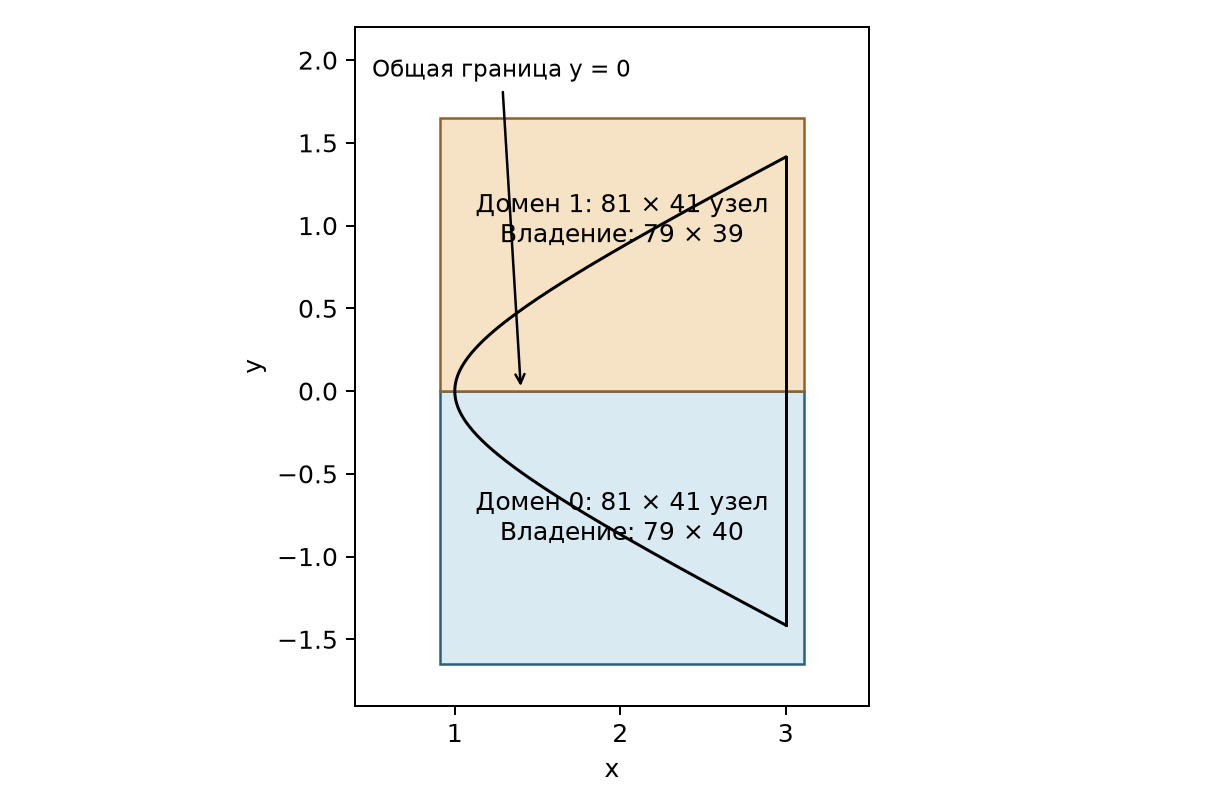
\includegraphics[width=0.71\textwidth]{decomposition.png}
\captionof{figure}{Сетка $80\times80$, два процесса. Граница $y=0$ общая
для доменов; интерфейсная неизвестная хранится у одного владельца.}
\end{center}
На сетке $80\times80$ два домена имеют по $81\times41$ узлу,
$81/41\approx1.97561<2$. Владение неизвестными остаётся $79\times40$
и $79\times39$; для него отношение $79/39>2$. Ранее критерий ошибочно
применялся к этому второму объекту. Здесь требование реализовано для
узлов замкнутых геометрических доменов; факт согласования такой
трактовки преподавателем не утверждается.

\clearpage
\section{Проверки корректности и эталон}
Проверки выполнены на нескольких независимых уровнях.
\begin{enumerate}
\item Геометрия: сумма $S_{ij}$ сравнивается с точной площадью $D$.
Первообразная, площадь, тождество для $J$ и свойства геометрического
разбиения дополнительно проверены в Mathematica.
\item Дискретная система заново собрана в Python: площади вычислены
численным интегрированием, а система собрана для $w$, без перехода
к поправке. Прямой решатель сравнивается с CG на $20^2$, $40^2$, $80^2$.
Максимальные расхождения составили $1.15\cdot10^{-13}$,
$3.48\cdot10^{-13}$ и $2.28\cdot10^{-12}$ соответственно.
\item Полные поля, включая границу, сравниваются между версиями на
сетках $80\times80$, $20\times30$, $19\times23$; после уточнения
декомпозиции добавлен пример $4\times6$. Проверяются также
некорректные аргументы, остановка по лимиту и ошибки записи.
\item Повреждение поля с сохранением его суммы должно провалить тест.
Это исключает прежний недостаток проверки одного интеграла.
\end{enumerate}

Восемь регрессионных групп прошли локально. Тест геометрии перебрал
38\,416 комбинаций сетки и числа процессов, проверяя покрытие области,
общие границы, отсутствие повторного владения и выбор допустимого
разложения. Допуск сравнения полных полей --- $10^{-10}$.

На Polus повторная проверка 3 ноября (LSF 1612342) прошла для всех
четырёх CPU-версий и CUDA на одной/двух GPU. Максимальное расхождение
полных полей с последовательной версией: CPU $2.22\cdot10^{-16}$,
CUDA $1.06\cdot10^{-13}$. Проверены также отказы расчёта и записи.

\subsection*{Эталон исходной краевой задачи}
В Mathematica задача решена методом конечных элементов непосредственно
в $D$, без фиктивной области. Использованы элементы второго порядка
и максимальные площади элемента $10^{-3}$, $2\cdot10^{-4}$,
$5\cdot10^{-5}$. Расчёт повторён 3 ноября; значения совпали с сохранённым
эталоном. В пяти точках максимальное изменение между двумя последними
сетками менее $2\cdot10^{-7}$. Это наблюдаемая устойчивость эталона,
а не доказанная оценка ошибки во всей области.

\begin{center}
\captionof{table}{Контрольные точки и значения FEM-эталона.}
\begin{tabular}{rrr}
\toprule $x$ & $y$ & $u_{\mathrm{FEM}}(x,y)$\\\midrule
2.0 & 0.0 & 0.791541548692\\
1.5 & 0.3 & 0.909701773896\\
2.5 & -0.8 & 0.915520114696\\
2.8 & 1.0 & -0.549224965113\\
1.2 & -0.2 & 0.815692173244\\\bottomrule
\end{tabular}
\end{center}
Для сравнения в этих точках применяется билинейная интерполяция
сеточного решения. Максимум по пяти точкам не называется
$C$-нормой ошибки во всей области. Сравнение с прямым решателем
подтверждает реализацию дискретной системы на проверенных сетках,
но само по себе не доказывает точность аппроксимации исходной задачи.

\clearpage
\section{Решение и сгущение сетки}
\begin{center}
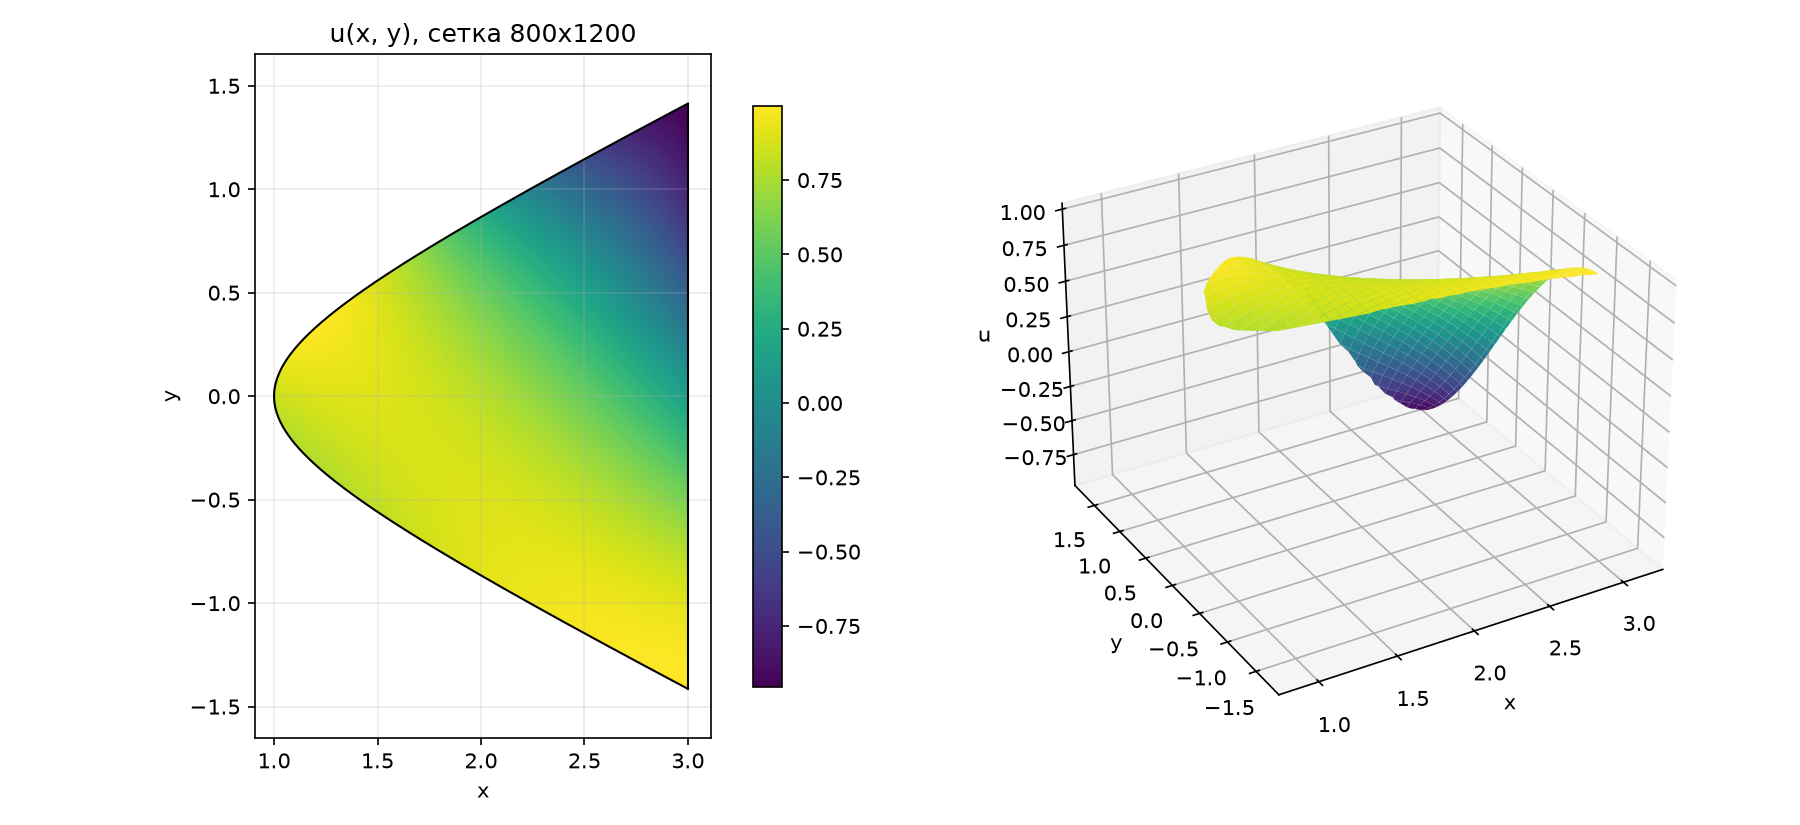
\includegraphics[width=\textwidth]{solution.png}
\captionof{figure}{Решение в области $D$ на сетке $800\times1200$ при
$\delta=10^{-6}$. Значения в фиктивной области не показаны.}
\end{center}
\begin{center}
\captionof{table}{Сходимость по сетке при штатном критерии остановки.
Последний столбец --- максимум отклонений от FEM в пяти точках.}
\small
\begin{tabular}{rrrr}
\toprule
Сетка & $h$ & Итераций & Ошибка в 5 точках\\
\midrule
$20\times20$ & 0.16500 & 31 & $3.84\cdot10^{-3}$\\
$40\times40$ & 0.08250 & 60 & $3.29\cdot10^{-3}$\\
$80\times80$ & 0.04125 & 113 & $2.79\cdot10^{-3}$\\
$400\times600$ & 0.00550 & 599 & $6.14\cdot10^{-4}$\\
$800\times1200$ & 0.00275 & 1018 & $4.04\cdot10^{-4}$\\
\bottomrule
\end{tabular}

\end{center}
\begin{center}
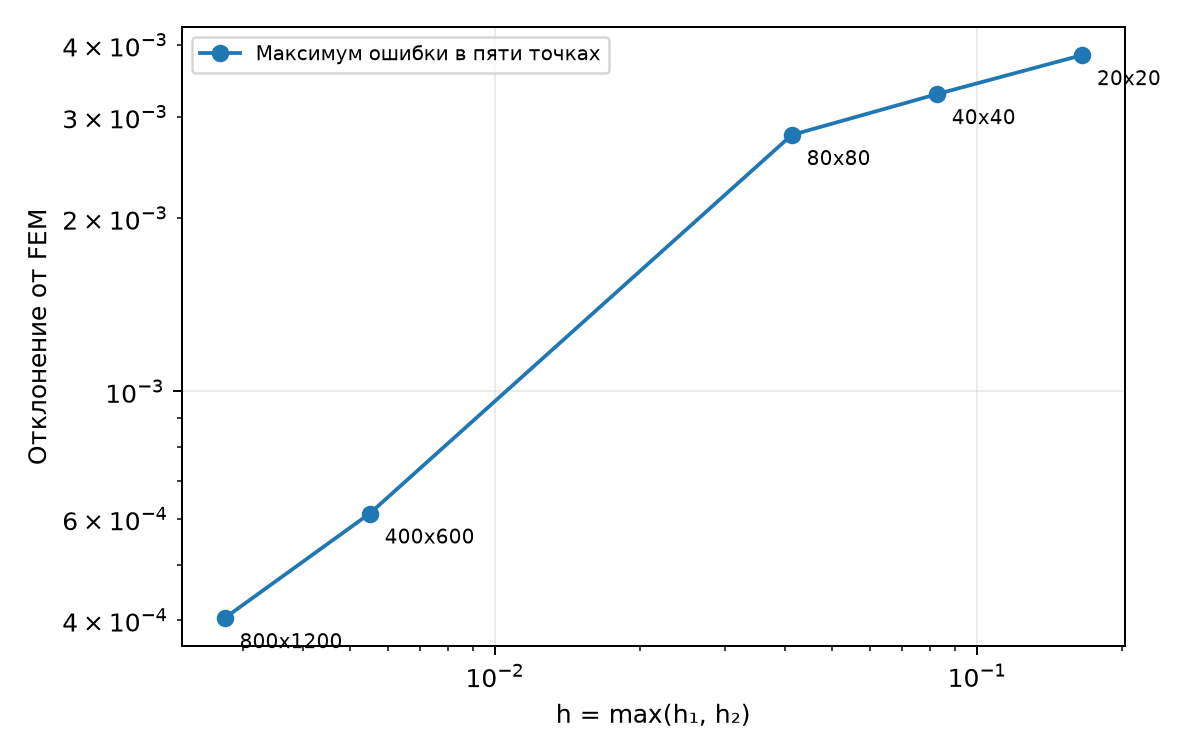
\includegraphics[width=0.56\textwidth]{grid_error.png}
\captionof{figure}{Изменение ошибки в контрольных точках при уменьшении
максимального шага. Изменяются и сетка, и параметр $\varepsilon=h^2$.}
\end{center}
По проверенным сеткам ошибка в точках уменьшается. Эти данные не
устанавливают асимптотический порядок метода. При $\varepsilon=h^2$
штраф в пересекаемых границей ячейках может иметь порядок $h^{-4}$;
эффект геометрии границы и итерационная ошибка требуют отдельного
контроля. Оценку для непрерывной задачи фиктивной области нельзя
автоматически переносить на дискретную схему с тем же порядком.

\clearpage
\section{Поитерационная сходимость}
Наблюдатель в диагностическом запуске читает текущее $d^{(k)}$ и отдельно
пересчитывает $Ad^{(k)}$. Он не изменяет векторы CG. Записываются начальная
точка и каждая итерация. Время диагностических запусков не включено
в таблицы ускорения. Совпадение конечного результата с обычным запуском
проверяется автоматически.

Сеточный эталон $\widetilde w_h$ вычислен той же схемой при
$\delta_{\mathrm{ref}}=10^{-13}$. Дополнительно выполнен расчёт с
$10^{-12}$; максимальное изменение поля не превысило
$1.26\cdot10^{-10}$. На трёх малых сетках эталон также сопоставлен с
прямым решателем. Это численный эталон, а не известное точное решение.

\begin{center}
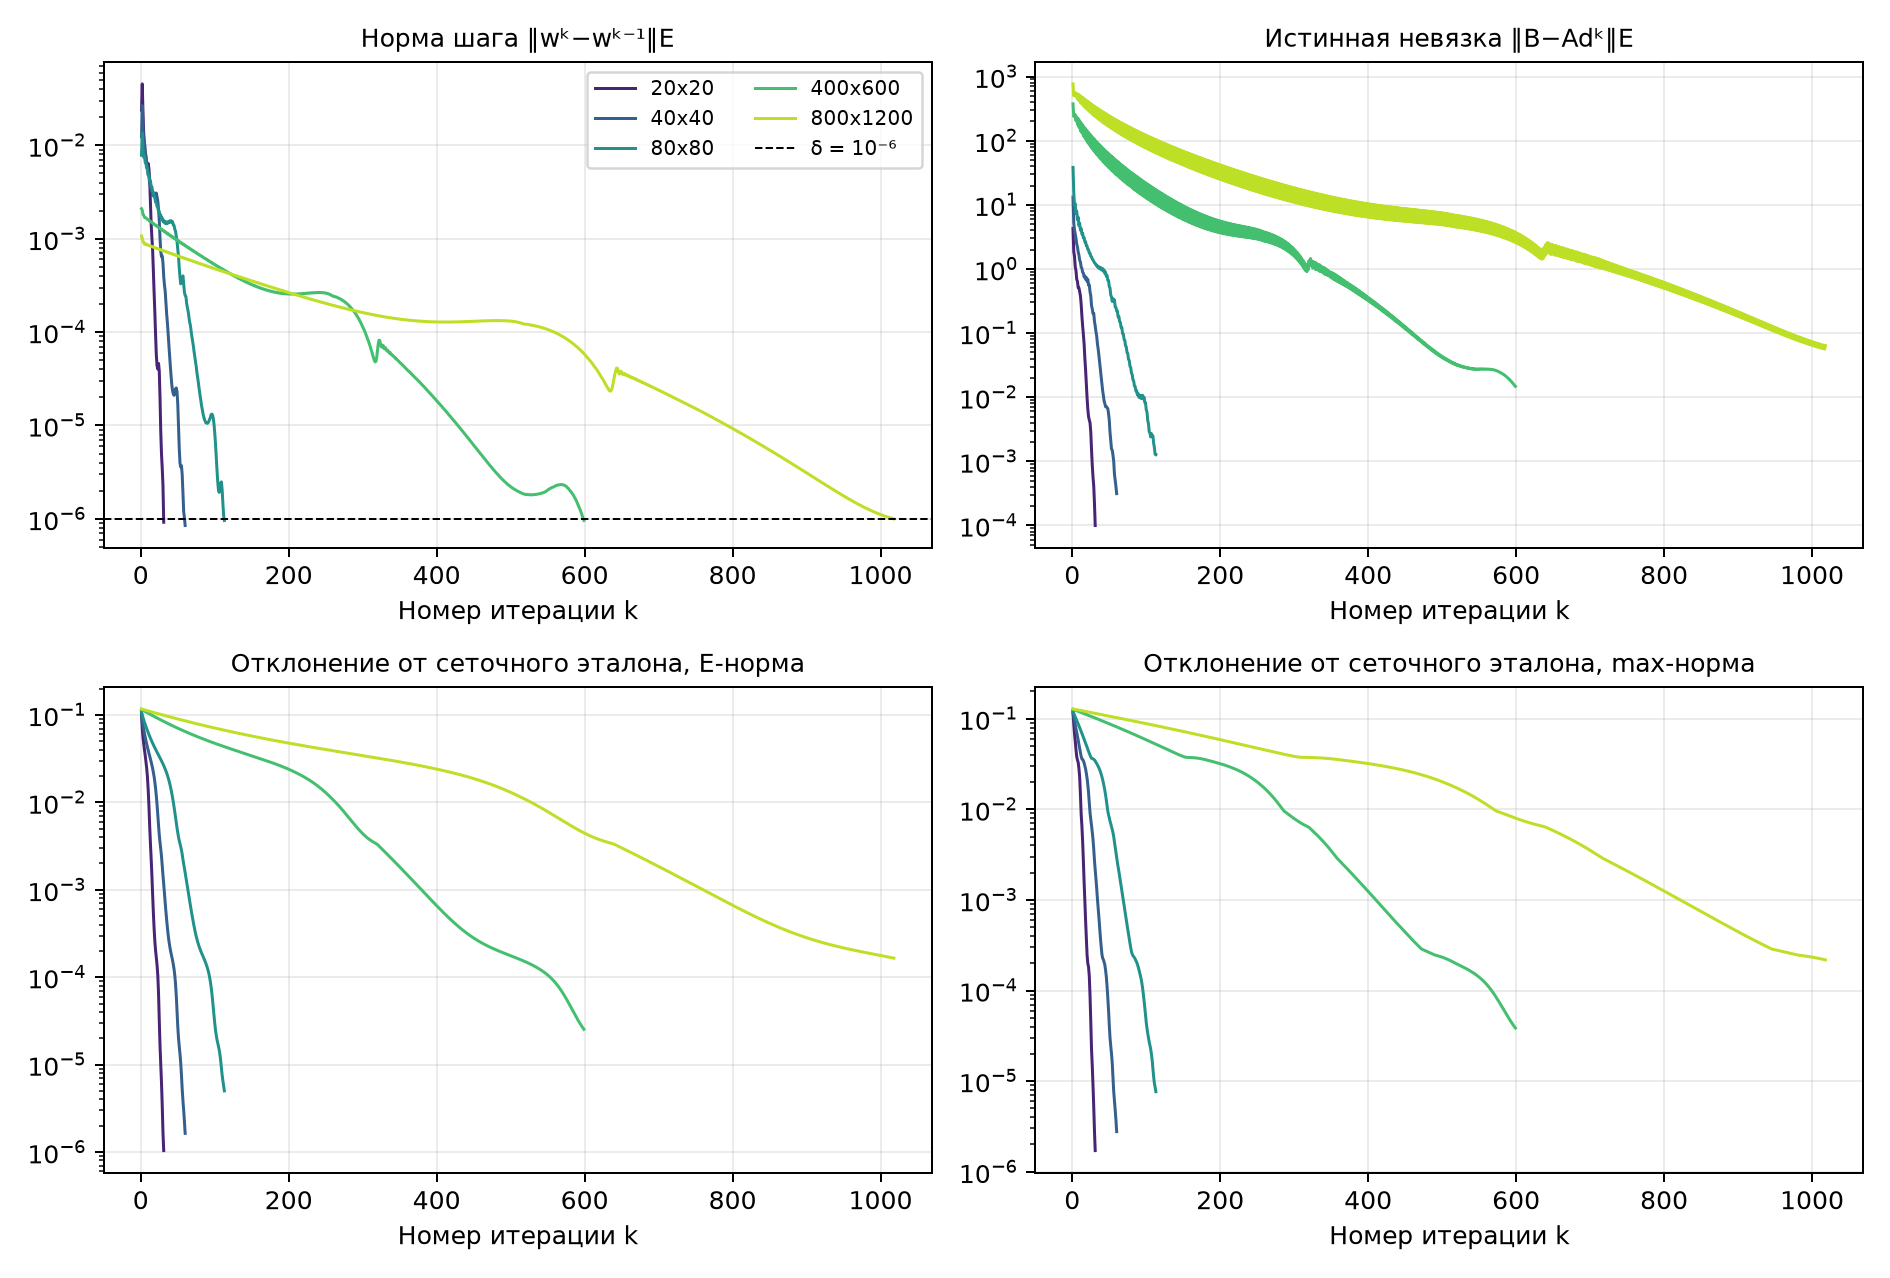
\includegraphics[width=\textwidth]{iterations.png}
\captionof{figure}{Четыре разные характеристики итераций. Сверху:
норма шага и заново вычисленная невязка. Снизу: ошибка относительно
$\widetilde w_h$ в $E$- и максимум-нормах по внутренним узлам $\Pi$.}
\end{center}
Использованы обозначения
\[
s_k=\norm{w^{(k)}-w^{(k-1)}}_\E,\quad
\rho_k=\norm{B-Ad^{(k)}}_\E,\quad
e_k=\norm{w^{(k)}-\widetilde w_h}_\E.
\]
При уменьшении шага число итераций растёт: от 31 на $20\times20$ до
1018 на $800\times1200$. Невязка и норма ошибки могут вести себя
немонотонно; контроль функционала не означает монотонности каждой из
этих величин. Во всех представленных трассах шаги приняты без перезапуска.

\clearpage
\section{Ошибка относительно FEM и выбор допуска}
\begin{center}
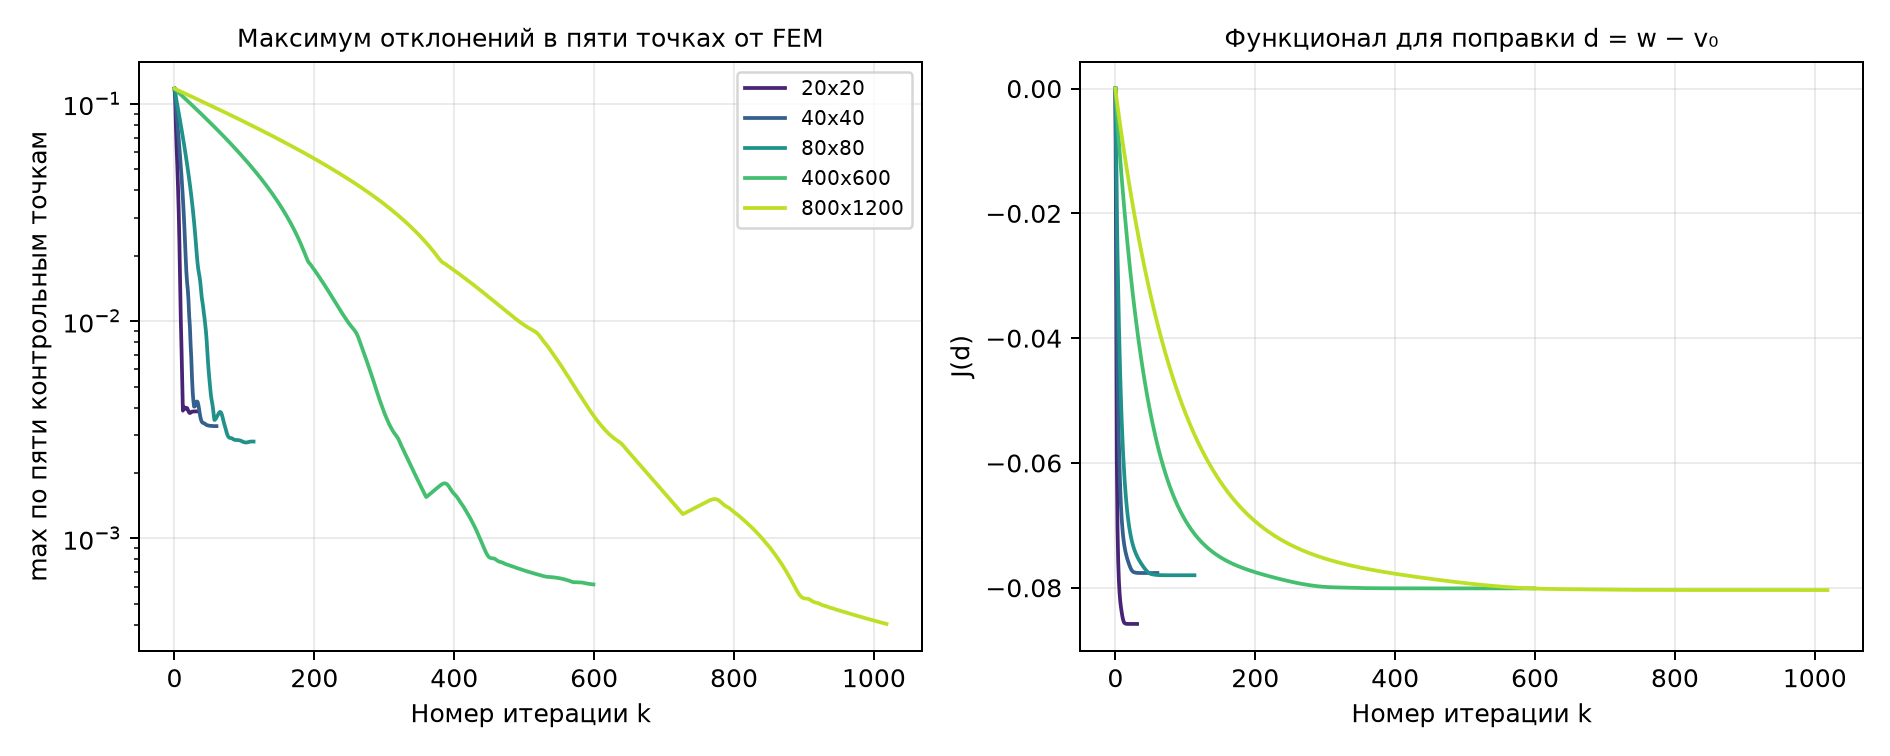
\includegraphics[width=\textwidth]{fem_and_functional.png}
\captionof{figure}{Слева --- максимум отклонений от FEM в пяти точках;
справа --- функционал $J(d^{(k)})$. Плато ошибки исходной задачи не равно
ошибке решения дискретной системы.}
\end{center}
\begin{center}
\captionof{table}{Характеристики в момент остановки при $\delta=10^{-6}$.}
\small
\begin{tabular}{rrrrr}
\toprule
Сетка & $s_k$ & $\rho_k$ & $e_k$ & $\|w^{(k)}-\widetilde w_h\|_\infty$\\
\midrule
$20\times20$ & $9.19\cdot10^{-7}$ & $9.99\cdot10^{-5}$ & $1.04\cdot10^{-6}$ & $1.71\cdot10^{-6}$\\
$40\times40$ & $8.48\cdot10^{-7}$ & $3.14\cdot10^{-4}$ & $1.64\cdot10^{-6}$ & $2.77\cdot10^{-6}$\\
$80\times80$ & $9.60\cdot10^{-7}$ & $1.27\cdot10^{-3}$ & $5.01\cdot10^{-6}$ & $7.64\cdot10^{-6}$\\
$400\times600$ & $9.61\cdot10^{-7}$ & $1.48\cdot10^{-2}$ & $2.54\cdot10^{-5}$ & $3.85\cdot10^{-5}$\\
$800\times1200$ & $9.99\cdot10^{-7}$ & $6.36\cdot10^{-2}$ & $1.65\cdot10^{-4}$ & $2.18\cdot10^{-4}$\\
\bottomrule
\end{tabular}

\end{center}
На самой мелкой сетке критерий $s_k<10^{-6}$ выполнен, однако
$\norm{w^{(k)}-\widetilde w_h}_\infty=2.18\cdot10^{-4}$, а
$\rho_k\approx6.36\cdot10^{-2}$. Следовательно, $\delta$ не следует
толковать как абсолютную погрешность поля или допуск по невязке.
Итерационная ошибка здесь сопоставима с отклонением от FEM.

В ранних заметках влияние $\delta$ оценивалось по изменению интеграла
решения. Интеграл может скрывать локальные отклонения; этот аргумент
недостаточен для вывода о малости ошибки поля. Настоящий отчёт заменяет
его прямым сравнением полных сеточных решений.

Функционал на разных сетках имеет разные предельные значения, поскольку
меняется дискретная задача. Убывание $J$ проверяется вдоль одной
итерационной последовательности; значения разных сеток не служат
межсеточным критерием качества.

\clearpage
\subsection*{Дополнительный опыт на сетке $800\times1200$}
\begin{center}
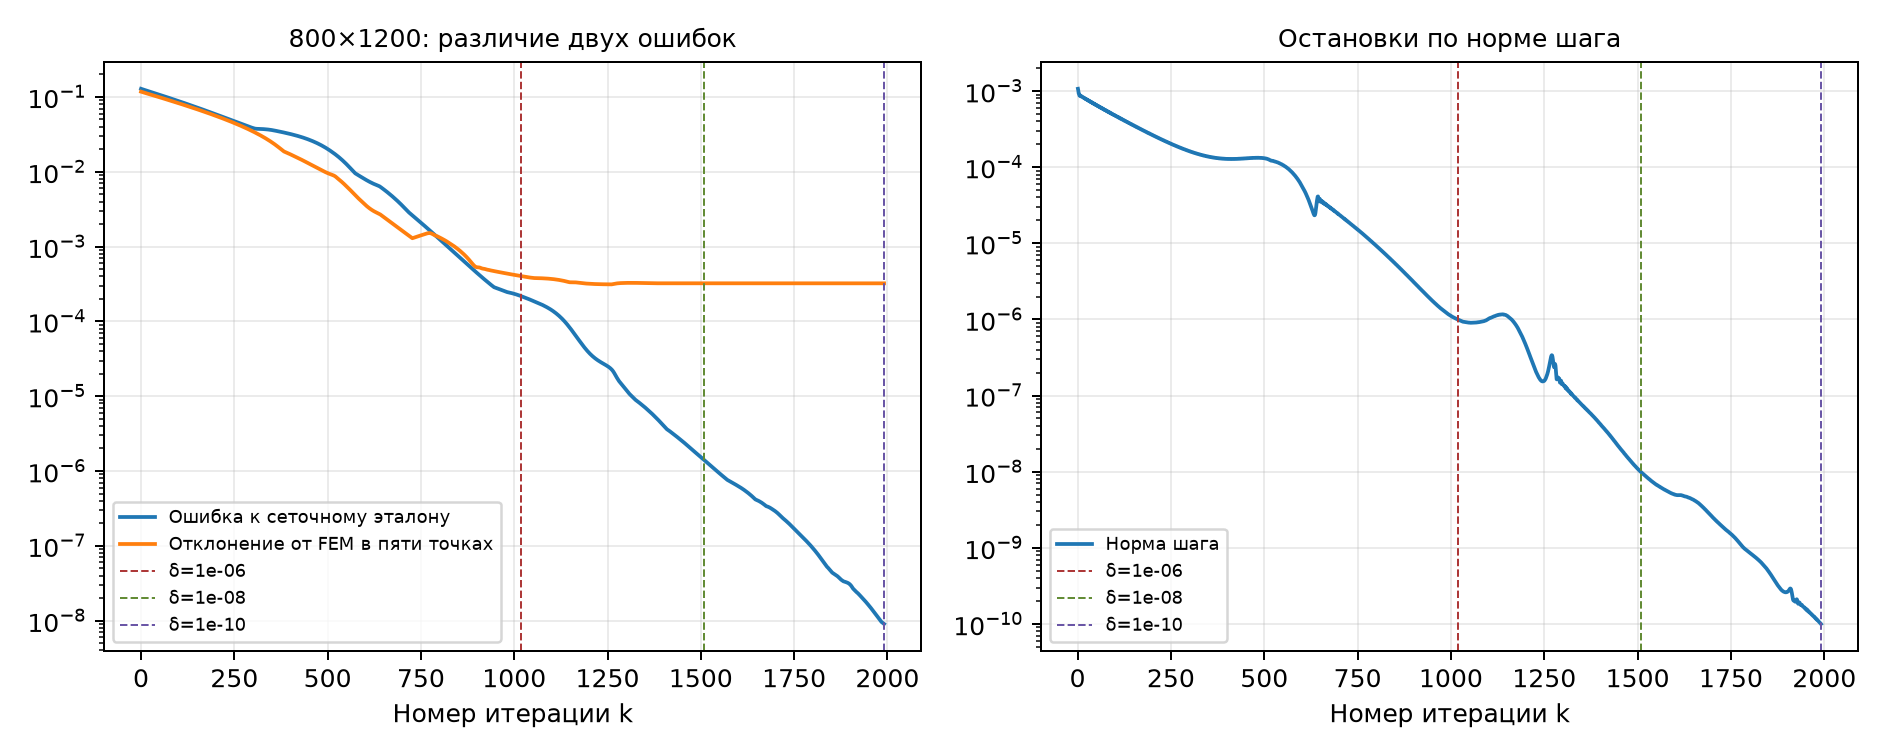
\includegraphics[width=\textwidth]{tolerance.png}
\captionof{figure}{Продолжение итераций до $\delta=10^{-10}$.
Вертикальные линии отмечают остановки при разных допусках.}
\end{center}
\begin{center}
\captionof{table}{Влияние допуска на число итераций и два разных вида ошибки.}
\small
\begin{tabular}{rrrr}
\toprule
$\delta$ & Итераций & Ошибка к сеточному эталону & Ошибка в 5 точках\\
\midrule
$1.00\cdot10^{-6}$ & 1018 & $2.18\cdot10^{-4}$ & $4.04\cdot10^{-4}$\\
$1.00\cdot10^{-8}$ & 1508 & $1.42\cdot10^{-6}$ & $3.23\cdot10^{-4}$\\
$1.00\cdot10^{-10}$ & 1991 & $9.03\cdot10^{-9}$ & $3.23\cdot10^{-4}$\\
$1.00\cdot10^{-13}$ & 2582 & $0$ & $3.23\cdot10^{-4}$\\
\bottomrule
\end{tabular}

\end{center}
За сеточный эталон принят запуск с $\delta=10^{-13}$, поэтому его
отклонение от самого себя равно нулю по определению. Отклонение от FEM
при этом сохраняется. Оно включает дискретизацию и фиктивную область,
а также погрешности FEM и интерполяции.

Для более точного поля на этой сетке следует использовать как минимум
проверенный режим \texttt{--delta 1e-8} и контролировать результат.
Основные таблицы производительности ниже относятся строго к исходному
$\delta=10^{-6}$; их нельзя выдавать за измерения при более строгом
допуске. Последовательность уточняющих запусков приведена отдельно,
так что точность и производительность не смешиваются.

\clearpage
\section{Производительность на Polus}
Основная серия 3 выполнена 4 октября 2026 года на узлах c3/c4 кластера
Polus с IBM POWER8. Сборка: IBM XL, параметры
\texttt{-O3 -qstrict -qarch=pwr8 -qtune=pwr8}; для OpenMP дополнительно
\texttt{-qsmp=omp}, для MPI используется Spectrum MPI.

На каждый опыт выполнено три повтора. Узлы выделялись монопольно
(\texttt{\#BSUB -x}); параметры привязки и размещения сохранены в LSF-файлах.
Время --- минимум трёх повторов, включает сборку коэффициентов и CG,
но не запись поля. Для MPI берутся максимальные по процессам времена
этапов и затем суммируются. В столбце разброса указано
$100(T_{\max}-T_{\min})/T_{\min}$; это не доверительный интервал.
Ускорение $S=T_{\mathrm{seq}}/T$ вычислено относительно последовательного
запуска на той же сетке и с тем же $\delta=10^{-6}$.

Последовательные базы: $0.7804$ с и 599 итераций на $400\times600$;
$5.3568$ с и 1018 итераций на $800\times1200$.
Далее воспроизведены исходные таблицы серии 3; ноябрьские проверки
корректности не подменяют эти измерения.

\begin{center}
\captionof{table}{OpenMP: таблица 1 задания.}
\small
\begin{tabular}{rrrrrr}
\toprule
Нитей & Сетка & Итер. & $T$, с & $S$ & Разброс\\
\midrule
2 & $400\times600$ & 599 & 0.3849 & 2.03 & 1\%\\
4 & $400\times600$ & 599 & 0.1870 & 4.17 & 1\%\\
8 & $400\times600$ & 599 & 0.1033 & 7.55 & 0\%\\
16 & $400\times600$ & 599 & 0.0575 & 13.57 & 1\%\\
4 & $800\times1200$ & 1018 & 1.3570 & 3.95 & 1\%\\
8 & $800\times1200$ & 1018 & 0.6893 & 7.77 & 1\%\\
16 & $800\times1200$ & 1018 & 0.3489 & 15.35 & 24\%\\
32 & $800\times1200$ & 1018 & 0.2971 & 18.03 & 1\%\\
\bottomrule
\end{tabular}

\end{center}
\begin{center}
\captionof{table}{MPI: таблица 2 задания.}
\small
\begin{tabular}{rrrrrr}
\toprule
Проц. & Сетка & Итер. & $T$, с & $S$ & Разброс\\
\midrule
2 & $400\times600$ & 599 & 0.3824 & 2.04 & 3\%\\
4 & $400\times600$ & 599 & 0.1895 & 4.12 & 1\%\\
8 & $400\times600$ & 599 & 0.0937 & 8.33 & 2\%\\
16 & $400\times600$ & 599 & 0.0516 & 15.11 & 1\%\\
4 & $800\times1200$ & 1018 & 1.3562 & 3.95 & 0\%\\
8 & $800\times1200$ & 1018 & 0.6910 & 7.75 & 11\%\\
16 & $800\times1200$ & 1018 & 0.3427 & 15.63 & 1\%\\
32 & $800\times1200$ & 1018 & 0.1634 & 32.78 & 1\%\\
\bottomrule
\end{tabular}

\end{center}

\clearpage
\begin{center}
\captionof{table}{MPI+OpenMP: таблица 3 задания. Число исполнителей равно
произведению числа процессов и нитей.}
\small
\begin{tabular}{rrrrrrr}
\toprule
Проц. & Нитей & Сетка & Итер. & $T$, с & $S$ & Разброс\\
\midrule
2 & 1 & $400\times600$ & 599 & 0.4133 & 1.89 & 12\%\\
2 & 2 & $400\times600$ & 599 & 0.2052 & 3.80 & 1\%\\
2 & 4 & $400\times600$ & 599 & 0.1170 & 6.67 & 1\%\\
2 & 8 & $400\times600$ & 599 & 0.0749 & 10.42 & 12\%\\
4 & 1 & $800\times1200$ & 1018 & 1.4227 & 3.77 & 2\%\\
4 & 2 & $800\times1200$ & 1018 & 0.8484 & 6.31 & 4\%\\
4 & 4 & $800\times1200$ & 1018 & 0.3675 & 14.58 & 10\%\\
4 & 8 & $800\times1200$ & 1018 & 0.2364 & 22.66 & 32\%\\
\bottomrule
\end{tabular}

\end{center}
\begin{center}
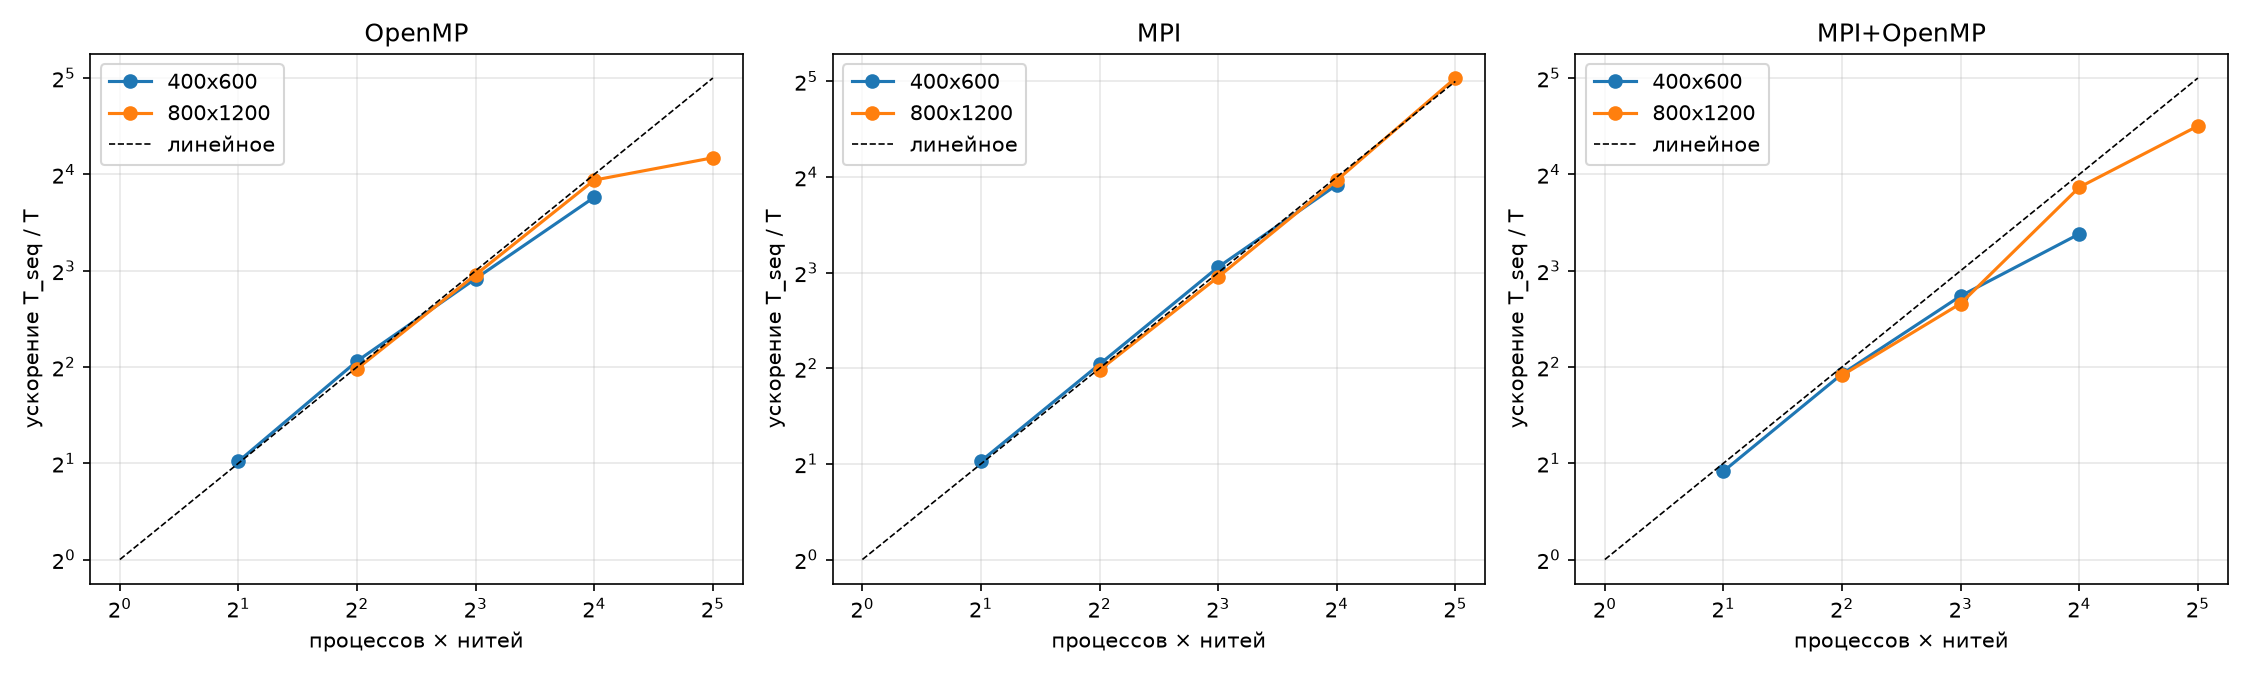
\includegraphics[width=\textwidth]{speedup.png}
\captionof{figure}{Ускорения из исходных логов серии 3. Пунктир ---
линейное ускорение; по оси абсцисс --- процессы, нити либо их произведение.}
\end{center}
OpenMP на $800\times1200$ даёт ускорение 15.35 на 16 нитях и 18.03 на
32 нитях. Прирост при дальнейшем увеличении числа нитей меньше;
точную причину нельзя установить только по этой таблице. В размещении
32 нитей использовались аппаратные нити одних и тех же физических ядер.

MPI даёт ускорение 15.63 на 16 процессах и 32.78 на 32 процессах.
Небольшое превышение линейного ускорения наблюдается, но его причина
не доказана: утверждение о влиянии кэша без отдельного опыта было отозвано.

Гибрид $4\times2$ на $800\times1200$ устойчиво уступает ожидаемому
масштабированию. Диагностика показывает дополнительное ожидание в
редукциях; гипотеза о попадании двух нитей на одно ядро была проверена
и не подтвердилась. Серия с \texttt{OMP\_WAIT\_POLICY} подготовлена,
но не выполнена; причина не объявляется установленной.

\clearpage
\section{История разработки и проверок}
\begin{description}[style=nextline,leftmargin=1em,labelwidth=0pt]
\item[Векторизация и OpenMP.]
Первоначально OpenMP-версия на одной нити была медленнее последовательной.
Диагностика компилятора показала отсутствие векторизации внутренних
циклов. Вычисления строки вынесены в функции со скалярными параметрами
и указателями \texttt{\_\_restrict\_\_}. После изменения времена одной
нити и последовательной версии сблизились.
\item[Положение прямоугольника.]
При $\Pi_x=(0.9,3.1)$ ошибка в контрольных точках почти не менялась
на сетках 20, 40 и 80. Общий для вложенных сеток узел вблизи $x=3$
оказывался в пересечённой ячейке. После сдвига до $(0.91,3.11)$
граница $x=3$ совпадает с узлом, и ошибка начала уменьшаться.
\item[Серия 1 на Polus.]
Замеры на узле c2 отличались от c3/c4: последовательный расчёт
$800\times1200$ занимал около 8.27 с против 5.0--5.1 с. Частоты и
доступные показатели нагрузки не позволили установить причину.
Дальнейшая серия ограничена узлами c3/c4, а исключение узла зафиксировано.
\item[Серии 2 и 3.]
Разброс повторов при совместной работе собственных заданий доходил
до 58\%. После перехода к монопольному выделению узла большинство
строк стабилизировалось. Сохранились отдельные выбросы, поэтому в
таблицах приведены и число повторов, и разброс, а не только минимум.
\item[Серия 4 и привязка.]
Проверка \texttt{OMP\_PLACES=cores} привела к сильному замедлению:
использованные места OpenMP не соответствовали выделенным процессу
ядрам. Для диагностики добавлен \texttt{--binding}; по пути исправлено
переполнение буфера имени узла. Неудачные запуски сохранены.
\item[Аудит перед сдачей.]
В ноябре исправлены ложный успех при недостигнутом критерии CG,
ошибка возврата статуса записи MPI, слабая валидация аргументов и
сравнение только интегралов. Добавлены проверки полных полей и
повреждённых данных. Ревью выявило также неверный вывод $J$ при точном
ненулевом начальном приближении; этот случай исправлен и покрыт тестом.
\item[Поитерационный контроль и домены.]
Добавлены независимый наблюдатель CG и сеточные эталоны с более строгим
допуском. Сравнение поля уточнило прежний вывод о влиянии $\delta$.
Критерий декомпозиции перенесён с уникальных неизвестных на узлы
замкнутых геометрических доменов; обе величины выводятся раздельно.
\end{description}
История в публичном репозитории выделена из каталога \texttt{task1}
исходного рабочего репозитория. Порядок, даты и авторство прежних
коммитов сохранены; хеши изменились при выделении подкаталога.
Искусственные ошибки или фиктивная история разработки не добавлялись.

\clearpage
\begingroup
\setstretch{1.03}
\small
\section{Воспроизведение и использование ИИ}
\subsection*{Воспроизведение результатов}
Для CPU-сборки нужны C++-компилятор, OpenMP и MPI. На macOS используется
clang с libomp и Open MPI; на Polus Makefile выбирает IBM XL.
Python-зависимости объявлены в заголовках скриптов и устанавливаются
через \texttt{uv}. Отчёт собирается XeLaTeX.
\begin{verbatim}
make -j4 all trace_cg
bash tests/run_local.sh
uv run tools/build_report_data.py --work-dir /path/to/work
wolframscript -file tests/verify_report.wls
bash report/build.sh
\end{verbatim}
CSV каждой итерации и численные сводки находятся в \path{report/data/};
скрипт повторно использует совпадающие по исходникам и аргументам
опорные расчёты. Графики и таблицы имеют машинно читаемые источники.
Замеры Polus воспроизводятся по заданиям \path{jobs/lsf/}; исходная
серия производительности хранится в \path{results/polus/s3/}.

\subsection*{Где использован ИИ}
Claude Code (Anthropic) 1 октября 2026 года нашёл вариант в материалах
курса, написал четыре CPU-версии, генератор заданий LSF, скрипты
проверки и сбора таблиц; выполнил локальные прогоны, диагностику
векторизации, выбор прямоугольника и первые проверки на Polus.
4 октября с его помощью проведены серии 1--4, проанализированы
медленный узел и конкуренция заданий. 8 октября подготовлена
дополнительная MPI+CUDA-версия и её проверки.

Codex 3 ноября 2026 года выполнил аудит с отдельным ревьюером,
подготовил публичный репозиторий, исправил программные дефекты,
добавил регрессионные тесты, поитерационную диагностику и уточнение
геометрического разбиения, организовал проверки Mathematica и Polus,
подготовил графики и текст настоящего отчёта. Использование ИИ не
скрывается и не заменяет требуемую на беседе способность автора
самостоятельно объяснить алгоритм, код и результаты.

\subsection*{Ограничения и выводы}
Основные четыре реализации решают одну и ту же дискретную систему;
совпадение подтверждено проверками полных полей. Таблицы демонстрируют
масштабирование на заданных конфигурациях, но не доказывают общую
модель производительности. Норма шага не равна погрешности решения;
выбор допуска должен учитывать именно ошибку поля.

Дополнительная CUDA-версия находится в отдельной ветке и проверена
на одной и двух GPU. В прочитанном условии задачи 1 CUDA отсутствует;
соответствие отдельному заданию для автомата этим отчётом не утверждается.
Согласование трактовок и окончательная приёмка происходят на сдаче.
Отправка отчёта преподавателю и отсчёт 48 часов не являются результатом
вычислительной проверки и в этом документе не удостоверяются.

\subsection*{Источники}
\begin{enumerate}
\item Мокин А. Ю. Задание по курсу «Суперкомпьютерное моделирование
и технологии», сентябрь 2026. Разделы 3--6 и таблицы 1--3.
Материалы получены через \url{https://edu-cmc-skmodel.sourcecraft.site/}.
\item Исходные программы и логи настоящей работы:
\url{https://github.com/Shirlineyn/skipod-task1-2026}.
\item Код независимых проверок: \path{tests/direct_check.py},
\path{tests/reference.wls}, \path{tests/verify_report.wls};
сохранённый FEM-эталон: \path{tests/reference.out}.
\end{enumerate}
\endgroup
\end{document}
